\chapter{Introduction}\label{ch:intro}

% TODO: replace Computer Vision with OCR -> make sure it's ok with citations
\section{Motivation}
Nowadays it is hard to find a business process that doesn't use software for improvement.
Various technologies come to be valued because of this.
A recent trend is to use Deep Learning for types of problems that range from self driving
cars to medical diagnosis~\cite{balas_handbook_2019}.
Deep Learning is a powerful technology based on Artificial Neural Networks where data is processed
in multiple layers to extract features and solve a given problem~\cite{shrestha_review_2019}.
One area where this is especially helpful is the field of Computer Vision.
Deep Learning for Computer Vision has only caught on in the recent years as the big computational
cost has been met by the improvement in computer hardware~\cite{ponti_everything_2017}.
Computer vision deals with extracting information from photos.
This includes tasks like recognizing faces or reading text~\cite{prince_computer_2012}.
Applying Deep Learning to extract equipment labels from photos fits right into this crease of
applying technology for making daily problems more efficient.
Combining the two fields to create value and learning about the underlying theoretical foundations
and inner workings is the motivating factor of this work.

\section{Problem description}\label{se:problem}
% TODO: add costs
% TODO: cut down this part -> put into EDA part
% TODO: define requirements better
Motivated by the wide success of Deep Learning concerning Computer Vision,
the objective of this work is to implement and train a Deep Learning model that can extract
equipment names from photos taken of name plates.

When determining whether automisation is an improvement four aspects have to be examined.
These are time, costs, quality and flexibility.
The aspects build a quadrangle that is based on the optimizing trade-off between the
factors~\cite{dumas_fundamentals_2013}.

Without software supporting the task of reading the name of the picture  and typing it into
the system, can take long seconds, whereas a trained Deep Learning model could complete the task
in a mere instant.
Therefor automisation via Deep Learning should improve the efficiency of the process when compared to
manually reading and typing the information off the image.

Training costs for a Deep Learning model are very high due to the computing intensive
backpropagation algorithm that tunes the network to the data.
But the usage cost is low.
For manual labor the opposite is the case as training a person to type in a label is done quickly
and labor costs are high in comparison to the expenses for running the model.

Both Deep Learning models and human labor are not 100\% accurate.
It is human to make mistakes and because Deep Learning is trained only trained on a specific set
of data it makes sense that not all predictions can be correct as there can always be outliers in
the data. % TODO: find source
The question is whether the model can be as accurate or even better than its human counterpart.
This is especially interesting when it is applied in the real world where it might have to do good
in subpar situations.
An example is bad image quality.

Flexibility is concerned with how well a process can adjust to changing requirements.
A set of new equipment names that have to be included can pose a problem to a Deep Learning model
because it is not trained for the new data.
A human on the other hand should not have any problems in this regard.

The main concern for the solution's efficacy is whether it is accurate enough.
Therefor this work focuses on this aspect in particular.

\section{Methodology}

The goal of this work is to implement and train a Deep Learning model to read in labels from photos.
The emerging artifact can be used to solve the problem detailed in~\ref{se:problem}.
The expository instantiation is helpful to gain more understanding the artifact as it is common
in design science.
In particular this is justificatory knowledge on the design on the Deep Learning model and
Machine Learning way of approaching problems.
This is important in order to apply it and to optimize existing research to the specific problem.

The methodology is based on action research~\cite{johannesson_introduction_2021}.
It constists of a cycle of five phases: Diagnosis, Planning, Intervention, Evaluation, Reflection.
% TODO: add how I get data
The first cycle will entail an exploratory data analysis which corresponds to the Diagnosis part.
Here it is important to recognize main characteristics of the images and to find outliers
and other potential problems~\cite{cox_translating_2017}.
The research is then extended to existing practical solutions for similar practical problems as
well as proposed architectures from academic research.
Theoretical knowledge about the models as well as practical information about results for
similar problems contribute to the discussion about which approach is the most promissing.
Combining architectures is also a viable possibility to solve the given problem.
This concludes the Planning phase and will lead to a model exaptation that evolves to be the
artifact at the center of this thesis.
The next step is implementing and training the chosen approach which.
Evaluation for of the current model follows.
Storing and analyzing results of training and cross validation as well as visualizing the training
progress is an important part of this.
In the Reflection stage it is decided whether a new cycle should be carried out.

From the second cycle on the first three phases change as there already is a model that is to be
improved.
This time the Diagnosis phase entails asking questions about the existing model: What worked?
Why did it work/not work? What needs to change?
Changes are planned and implemented accordingly.
The Evaluation and Reflection phases are not changing in the second cycle thus closing the loop.
The incremental adjustments to the model are made in order to improve the accuracy.
This includes possibly adjusting the architecture, hyperparameter tuning and preprocessing approaches
like image compression.

\section{Expected results and outlook}
The research into the theoretical foundation of Deep Learning and into possible approaches leads
to a strong understanding of the underlying technology.
This is helpful to produce a comparison of approaches that is based on theoretical as well as
practical knowledge.
The goal is to find out which approach work best for the chosen practical problem and why that is the
case.
Implementation and training of the most promissing one is yielding the artifact this work revolves
around.
The process of optimization not only improves the solution to the problem (see~\ref{se:problem}) but
is also used to learn more about the implemented approach.

Integrating the artifact into the business process is not an issue that is discussed in
this work.
Nor will model feedback and over time iteration be part.

The intendet structure of the thesis with dependencies between chapters can be found in
figure~\ref{fig:chapters}.

\begin{figure}[ht]
    \centering
    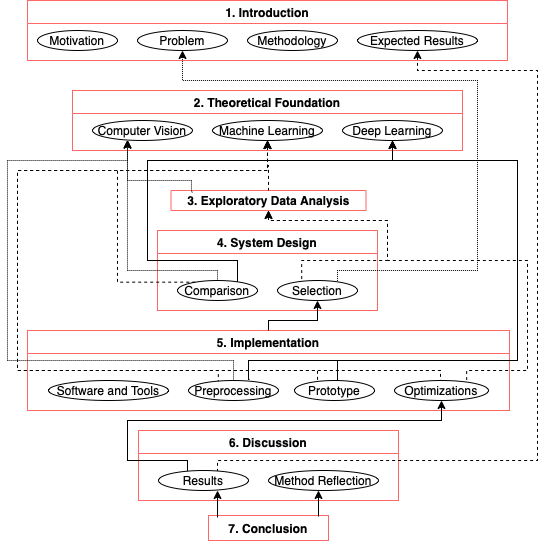
\includegraphics[width=1.0\textwidth]{img/Chapter.drawio.png}
    \caption{Chapters with subchapters and dependencies\label{fig:chapters}}
\end{figure}
